\documentclass[a4paper,10pt,twoside]{article}

\usepackage[top=1in, bottom=1in, left=1in, right=1in]{geometry}
\usepackage[utf8]{inputenc}
\usepackage[spanish,es-ucroman,es-noquoting]{babel}
\usepackage{setspace}
\usepackage{fancyhdr}
\usepackage{lastpage}
\usepackage{amsmath}
\usepackage{amsfonts}
\usepackage{verbatim}
\usepackage{listings}
\usepackage{graphicx}
\usepackage{float}
\usepackage{algorithmic}
\usepackage{color}
\usepackage{hyperref}
\usepackage[usenames,dvipsnames]{xcolor}
\definecolor{dkgreen}{rgb}{0,0.6,0}
\definecolor{gray}{rgb}{0.97,0.97,0.97}
\definecolor{mauve}{rgb}{0.58,0,0.82}
\usepackage{tikz}
\usetikzlibrary{calc}
\usetikzlibrary{decorations.pathreplacing}
\usepackage{ragged2e}

\lstset{
    backgroundcolor=\color{lbcolor},
    tabsize=4,
    rulecolor=,
    language=matlab,
        basicstyle=\scriptsize,
        upquote=true,
        aboveskip={1.5\baselineskip},
        columns=fixed,
        showstringspaces=false,
        extendedchars=true,
        breaklines=true,
        prebreak = \raisebox{0ex}[0ex][0ex]{\ensuremath{\hookleftarrow}},
        frame=single,
        showtabs=false,
        showspaces=false,
        showstringspaces=false,
        identifierstyle=\ttfamily,
        keywordstyle=\color[rgb]{0,0,1},
        commentstyle=\color[rgb]{0.133,0.545,0.133},
        stringstyle=\color[rgb]{0.627,0.126,0.941},
}

% Evita que el documento se estire verticalmente para ocupar
% el espacio vacío en cada página.
\raggedbottom


%%%%%%%%%% Configuración de Fancyhdr - Inicio %%%%%%%%%%
\pagestyle{fancy}
\thispagestyle{fancy}
\lhead{Trabajo Práctico Final, Organización del Computador II}
\rhead{DeliriOS}
\renewcommand{\footrulewidth}{0.4pt}
\cfoot{\thepage /\pageref{LastPage}}

\fancypagestyle{caratula} {
   \fancyhf{}
   \cfoot{\thepage /\pageref{LastPage}}
   \renewcommand{\headrulewidth}{0pt}
   \renewcommand{\footrulewidth}{0pt}
}
%%%%%%%%%% Configuración de Fancyhdr - Fin %%%%%%%%%%


%%%%%%%%%% Configuración de Algorithmic - Inicio %%%%%%%%%%
% Entorno propio para customizar la presentación del pseudocódigo
\newenvironment{pseudocodigo}
    {\vspace{0.5em} \begin{algorithmic}}
    {\end{algorithmic} \vspace{0.5em}}

% Alinear comentarios a la derecha
\renewcommand{\algorithmiccomment}[1]{\hfill \{#1\}}
%%%%%%%%%% Configuración de Algorithmic - Fin %%%%%%%%%%


%%%%%%%%%% Macros de tikz - Inicio %%%%%%%%%%
% Uso: \registroCuatro{etiqueta}{x}{y}{a4}{a3}{a2}{a1}
\newcommand{\registroCuatro}[7]{
    \ifthenelse{\equal{#1}{}}{}{
        \draw (#2, {#3 + 0.5}) node[anchor=east]{#1};
    }

    \draw   (#2, #3) rectangle +(4, 1) +(2, 0.5) node{#4}
          ++(4, 0)   rectangle +(4, 1) +(2, 0.5) node{#5}
          ++(4, 0)   rectangle +(4, 1) +(2, 0.5) node{#6}
          ++(4, 0)   rectangle +(4, 1) +(2, 0.5) node{#7};          
}

% Uso: \registroOcho{etiqueta}{x}{y}{a8}{a7}{a6}...{a1}
\newcommand{\registroOcho}[9]{
    \def\etiqueta{#1}
    \def\x{#2}
    \def\y{#3}
    \def\aviii{#4}
    \def\avii{#5}
    \def\avi{#6}
    \def\av{#7}
    \def\aiv{#8}
    \def\aiii{#9}
    \registroOchoX    
}
\newcommand{\registroOchoX}[2]{ % Auxiliar - no usar directamente
    \def\aii{#1}
    \def\ai{#2}
    \ifthenelse{\equal{\etiqueta}{}}{}{
        \draw (\x, {\y + 0.5}) node[anchor=east]{\etiqueta};
    }
    \filldraw[fill=white]
        (\x, \y) rectangle +(2, 1) +(1, 0.5) node{\aviii}
        ++(2, 0) rectangle +(2, 1) +(1, 0.5) node{\avii}
        ++(2, 0) rectangle +(2, 1) +(1, 0.5) node{\avi}
        ++(2, 0) rectangle +(2, 1) +(1, 0.5) node{\av}
        ++(2, 0) rectangle +(2, 1) +(1, 0.5) node{\aiv}
        ++(2, 0) rectangle +(2, 1) +(1, 0.5) node{\aiii}
        ++(2, 0) rectangle +(2, 1) +(1, 0.5) node{\aii}
        ++(2, 0) rectangle +(2, 1) +(1, 0.5) node{\ai};
}


% Uso: \registroDieciseis{etiqueta}{x}{y}{a16}{a15}{a14}...{a1}
\newcommand{\registroDieciseis}[9]{
    \def\etiqueta{#1}
    \def\x{#2}
    \def\y{#3}
    \def\axvi{#4}
    \def\axv{#5}
    \def\axiv{#6}
    \def\axiii{#7}
    \def\axii{#8}
    \def\axi{#9}
    \registroDieciseisX
}
\newcommand{\registroDieciseisX}[9]{ % Auxiliar - no usar directamente
    \def\ax{#1}
    \def\aix{#2}
    \def\aviii{#3}
    \def\avii{#4}
    \def\avi{#5}
    \def\av{#6}
    \def\aiv{#7}
    \def\aiii{#8}
    \def\aii{#9}
    \registroDieciseisXX
}
\newcommand{\registroDieciseisXX}[1]{ % Auxiliar - no usar directamente
    \def\ai{#1}
    \ifthenelse{\equal{\etiqueta}{}}{}{
        \draw (\x, {\y + 0.5}) node[anchor=east]{\etiqueta};
    }
    \filldraw[fill=white]
        (\x, \y) rectangle +(1, 1) +(0.5, 0.5) node{\axvi}
        ++(1, 0) rectangle +(1, 1) +(0.5, 0.5) node{\axv}
        ++(1, 0) rectangle +(1, 1) +(0.5, 0.5) node{\axiv}
        ++(1, 0) rectangle +(1, 1) +(0.5, 0.5) node{\axiii}
        ++(1, 0) rectangle +(1, 1) +(0.5, 0.5) node{\axii}
        ++(1, 0) rectangle +(1, 1) +(0.5, 0.5) node{\axi}
        ++(1, 0) rectangle +(1, 1) +(0.5, 0.5) node{\ax}
        ++(1, 0) rectangle +(1, 1) +(0.5, 0.5) node{\aix}
        ++(1, 0) rectangle +(1, 1) +(0.5, 0.5) node{\aviii}
        ++(1, 0) rectangle +(1, 1) +(0.5, 0.5) node{\avii}
        ++(1, 0) rectangle +(1, 1) +(0.5, 0.5) node{\avi}
        ++(1, 0) rectangle +(1, 1) +(0.5, 0.5) node{\av}
        ++(1, 0) rectangle +(1, 1) +(0.5, 0.5) node{\aiv}
        ++(1, 0) rectangle +(1, 1) +(0.5, 0.5) node{\aiii}
        ++(1, 0) rectangle +(1, 1) +(0.5, 0.5) node{\aii}
        ++(1, 0) rectangle +(1, 1) +(0.5, 0.5) node{\ai};
}
%%%%%%%%%% Macros de tikz - Fin %%%%%%%%%%


%%%%%%%%%% Macros misceláneos - Inicio %%%%%%%%%%
\newcommand{\xmm}[1]{\texttt{XMM#1}}
\newcommand{\rax}{\texttt{RAX}}
\newcommand{\rbx}{\texttt{RBX}}
\newcommand{\rcx}{\texttt{RCX}}
\newcommand{\rdx}{\texttt{RDX}}
\newcommand{\rbp}{\texttt{RBP}}
\newcommand{\rsp}{\texttt{RSP}}
\newcommand{\reg}[1]{\texttt{R#1}}
\newcommand{\asm}[1]{\texttt{\uppercase{#1}}}
%%%%%%%%%% Macros misceláneos - Fin %%%%%%%%%%


\begin{document}


%%%%%%%%%%%%%%%%%%%%%%%%%%%%%%%%%%%%%%%%%%%%%%%%%%%%%%%%%%%%%%%%%%%%%%%%%%%%%%%
%% Carátula                                                                  %%
%%%%%%%%%%%%%%%%%%%%%%%%%%%%%%%%%%%%%%%%%%%%%%%%%%%%%%%%%%%%%%%%%%%%%%%%%%%%%%%


\thispagestyle{caratula}

\begin{center}


\includegraphics[height=2cm]{DC.png} 
\hfill

\includegraphics[height=2cm]{UBA.jpg} 

\vspace{2cm}

Departamento de Computación,\\
Facultad de Ciencias Exactas y Naturales,\\
Universidad de Buenos Aires

\vspace{4cm}

\begin{Huge}
Trabajo Práctico Final: DeliriOS
\end{Huge}

\vspace{0.5cm}

\begin{Large}
Organización del Computador II
\end{Large}

\vspace{1cm}

Marzo 2014

\vspace{4cm}

\begin{tabular}{|c|c|c|}
    \hline
    Apellido y Nombre & LU & E-mail\\
    \hline
    Silvio Vileriño             & 106/12 & svilerino@gmail.com\\
    Ezequiel Gambaccini 		& xxx/xx & xxx@xxx.com\\
    \hline
\end{tabular}

\vspace{1cm}


\end{center}
\newpage


%%%%%%%%%%%%%%%%%%%%%%%%%%%%%%%%%%%%%%%%%%%%%%%%%%%%%%%%%%%%%%%%%%%%%%%%%%%%%%%
%% Índice                                                                    %%
%%%%%%%%%%%%%%%%%%%%%%%%%%%%%%%%%%%%%%%%%%%%%%%%%%%%%%%%%%%%%%%%%%%%%%%%%%%%%%%

\tableofcontents

\newpage

    %%%%%%%%%%%%%%%%%%%%%%%%%%%%%%%%%%%%%%%%%%%%%%%%%%%%%%%%%%%%%%%%%%%%%%%%%%%%%%%
    %% Introduccion                                                              %%
    %%%%%%%%%%%%%%%%%%%%%%%%%%%%%%%%%%%%%%%%%%%%%%%%%%%%%%%%%%%%%%%%%%%%%%%%%%%%%%%
    \section{Introduccion}
    El objetivo de este trabajo práctico fue inicialmente experimentar con la arquitectura intel, realizando un microkernel de 64 bits inicializando multinúcleo. Más tarde en el desarrollo del proyecto se decidió extender el alcance del mismo, realizando algunos experimentos para analizar las posibles mejoras de rendimiento de algoritmos que se pueden paralelizar en varios núcleos, asimismo se realizaron varios enfoques diferentes en la sincronizacion entre núcleos: espera activa haciendo polling a memoria versus sincronizacion con interrupciones inter-núcleo que evitan los accesos al bus de memoria. La ganancia que esperamos obtener, es una reducción considerable en el overhead que genera el manejo de varios hilos sobre sistemas operativos utilizando librerias como por ejemplo pthreads, y de esta forma poder determinar si podría aprovecharse de mejor manera el hardware disponible para resolver problemas de mayor tamaño que el que nos permiten las librerias actuales para multihilo.
    \\

    El informe estará dividido en secciones, cada una describiendo una parte del trabajo.

    \newpage

    %%%%%%%%%%%%%%%%%%%%%%%%%%%%%%%%%%%%%%%%%%%%%%%%%%%%%%%%%%%%%%%%%%%%%%%%%%%%%%%
    %% Desarrollo                                                                %%
    %%%%%%%%%%%%%%%%%%%%%%%%%%%%%%%%%%%%%%%%%%%%%%%%%%%%%%%%%%%%%%%%%%%%%%%%%%%%%%%
    \section{Desarrollo: Inicialización y contexto del sistema}
            \subsection{Estructura de carpetas: Compilación, Linkeo y Scripts}
    \begin{itemize}
	    \item \textbf{ap code: } Contiene el código de los Application processors, tanto de inicialización desde modo protegido como de los algoritmos implementados.
		\item \textbf{ap startup code: } Contiene el código de inicializacion en modo real de los Application processors
		\item \textbf{bsp code: } Contiene el código de inicializacion del kernel, los algoritmos implementados, y el encendido de los Application Processors.
		\item \textbf{common code: } Contiene el código comun al Bootstrap Processor y los Application Processors.
		\item \textbf{grub init: } Contiene scripts y archivos de configuracion de grub, en la subcarpeta src se encuentra el loader que realiza el pasaje entre la máquina en especificación multiboot a modo largo de 64 bits.
		\item \textbf{run.sh: } Script para compilación y distribución del tp.
		\item \textbf{macros: } Esta carpeta contiene macros utilizadas en el código.
		\item \textbf{informe: } Contiene el informe del trabajo práctico en formato Latex y PDF.
		\item \textbf{include: } Contiene las cabeceras de las librerias.
    \end{itemize}

    El tp está compilado en varios archivos, de esta forma cargamos algunas partes como módulos de grub.
    Hay scripts encargados de compilar todo lo necesario, cada módulo tiene su Makefile y el comando make es llamado
    oportunamente por los scripts en caso de ser necesario.
    \\
    \\
    El linkeo está realizado con linking scripts en las carpetas donde sea necesario,
    cada seccion esta alineada a 4k por temas de compatibilidad, asimismo hay símbolos que pueden ser leidos desde el codigo si es necesario saber la ubicación de estas secciones en memoria.
    Los módulos de 32 bits estan compilados en elf32 y los de 64 bits en binario plano de 64 bits, esto es por temas de compatibilidad de grub al cargar modulos.
    \\
    \\
    Para correr el trabajo practico unicamente hace falta tipear $./run.sh -r$ en consola y se abrira en bochs el trabajo practico.
    
        \newpage
        	 \subsection{Integración con grub y división en módulos}

	Utilizamos grub en el nivel mas bajo del booteo para lograr un contexto inicial estable y que posibilitara la ejecución del trabajo practico desde un pendrive usb.\\

	Grub permite iniciar un kernel por medio de una especificación publicada en la web, en la que se detalla un contrato que debe cumplir tanto el kernel a iniciar como grub, entre ellas, un header que debe contener el ejecutable del kernel para ser identificado por grub como un sistema operativo, y por otro lado, las obligaciones que debe cumplir grub al entregarle el control a dicho kernel, es decir, un contexto determinado: selectores de código y datos válidos, registros de propósito general con valores específicos, etc.\\
	(\url{http://www.gnu.org/software/grub/manual/multiboot/multiboot.html})\\

	Esta revisión de grub no permite cargar ejecutables compilados en 64 bits de manera sencilla, por este motivo decidimos que lo mejor era utilizar a una herramienta provista por grub, llamada carga de módulos, que nos permitió cargar distintas partes no críticas del sistema por encima del primer mega de memoria y tener en un mapa de memoria provisto por grub, las posiciones exactas en la RAM de dichos módulos.\\ 

	Junto con la carga de módulos y el booteo del BSP, se prepara el entorno para el booteo en etapas de los AP.\\
	\begin{itemize}
		\item \textbf{Niveles de booteo del BSP y preparación del entorno de inicio de los AP:} 
			\begin{enumerate}
				\item Grub inicializa la máquina a un estado conocido y otorga el control al loader de nivel 1 del BSP pasándole por parámetros estructuras de grub con información del sistema.
				\begin{enumerate}
					\item Se realizan validaciones requeridas por la especificación multiboot, verificación de firmas, etc.
					
					\item Se obtienen de la metadata provista por grub las posiciones de memoria donde están cargados los módulos, ellos son:
					\vspace{0.1cm}
					\begin{description}
						\item [kernel64.bin64:] \hfill \\
							Módulo compilado en formato binario plano de 64 bits que contiene el segundo nivel de booteo del BSP.
						\item [ap\_full\_code.bin64:] \hfill \\
							Módulo compilado en formato binario plano de 64 bits que contiene el código del segundo nivel de booteo de los Application Processors.
						\item [ap\_startup\_code:] \hfill \\
							Módulo compilado en formato binario de 32 bits que contiene el código de inicio del AP en modo real y el primer stage de booteo a modo protegido.
					\end{description}
					\vspace{0.5cm}
					
					\item Los Application Processors inician en modo real, es por esto que deben comenzar su ejecución por debajo del primer mega de memoria principal. Por este motivo se copia el módulo ap\_startup\_code a una dirección arbitraria alineada a página 0x2000.
					\vspace{0.1cm}
					\item Como los AP comienzan su ejecución por debajo del primer mega, esto hace posible la superposición de código con grub y otras estructuras del kernel, para evitarlo, minimizamos el tamaño del startup de modo real del ap, haciendo lo antes posible un salto a un loader de nivel 2 por encima del mega, este loader de nivel 2 es ap\_full\_code.bin64.
					\vspace{0.1cm}
					\item Al tener el Application Processor que hacer un salto entre los dos niveles de booteo, se le inyecta al primer módulo la dirección donde esta cargado el segundo nivel de booteo.
					\vspace{0.1cm}
					\item Finalmente, se realiza un salto en la ejecución a donde comienza el modulo kernel64.bin64 donde el BSP finaliza la inicializacion del contexto hasta modo largo de 64 bits y enciende a los demás núcleos del sistema.
				\end{enumerate}
			\end{enumerate}
	\end{itemize}

	\subsubsection{Booteo e integración con grub: Mapa de memoria: Memoria baja y módulos en memoria alta}

	\begin{center}
		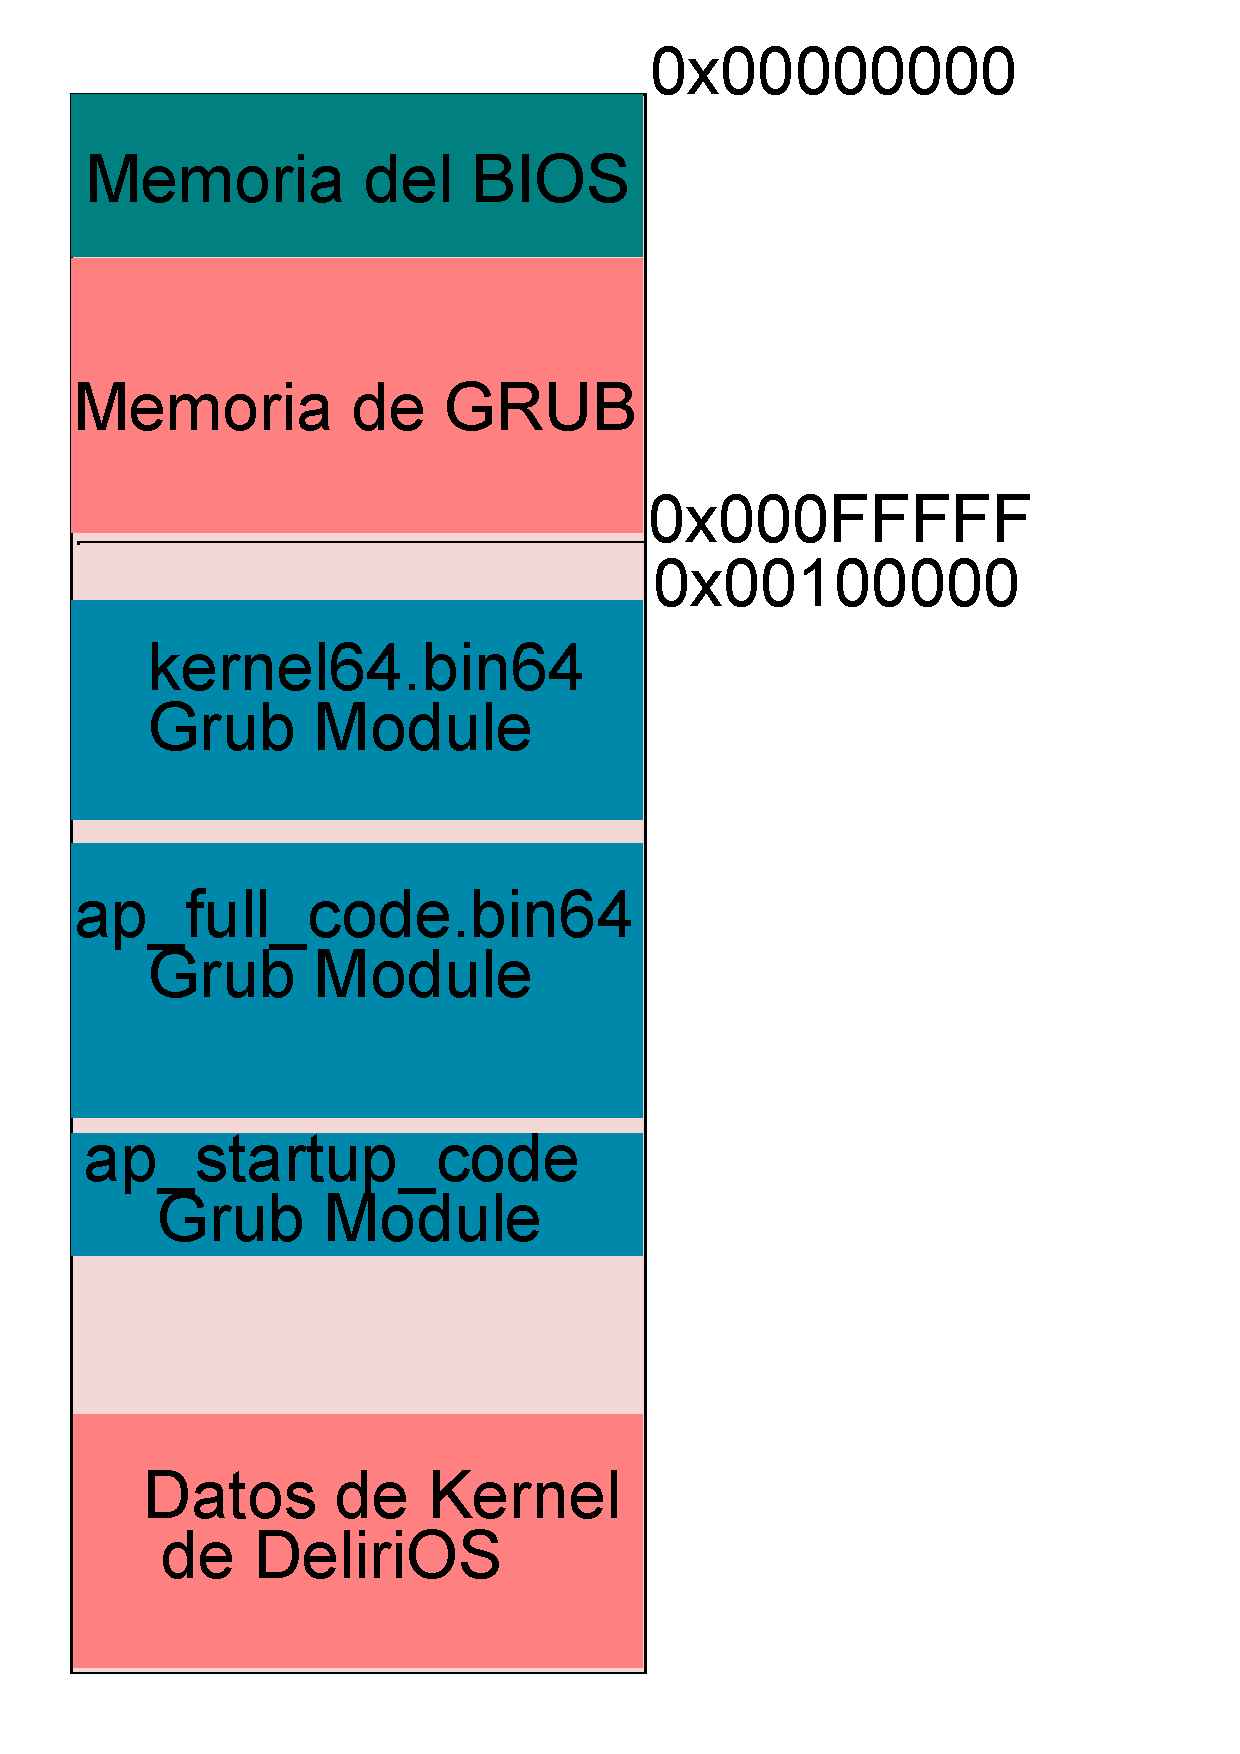
\includegraphics[height=7cm]{images/modules-map.pdf} 
	\end{center}
	\subsubsection{Booteo e integración con grub: Diagrama de interacción entre los niveles de Booteo e inyección de datos}

	\begin{center}
		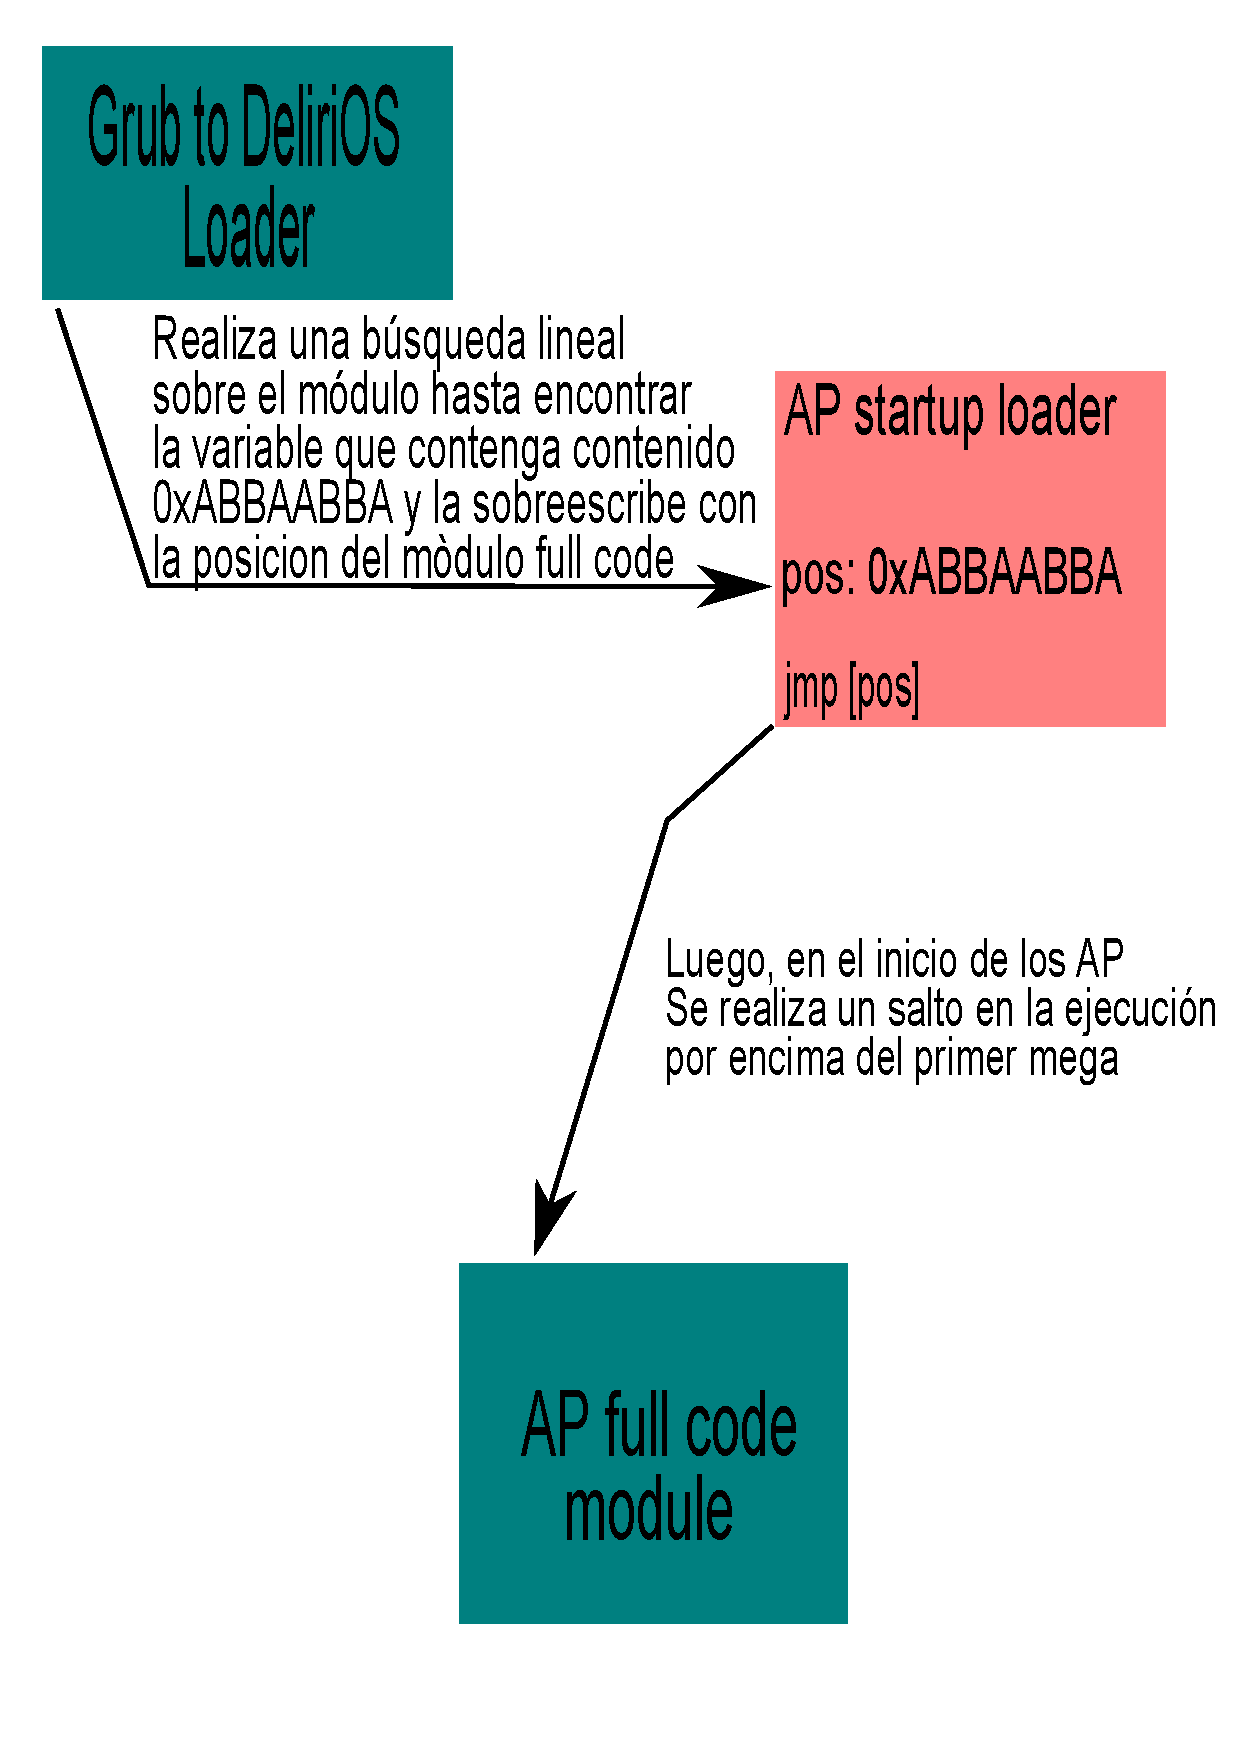
\includegraphics[height=12cm]{images/modules-diagram.pdf} 
	\end{center}

	\newpage

	\subsubsection{Niveles de booteo del BSP}

	\begin{center}
		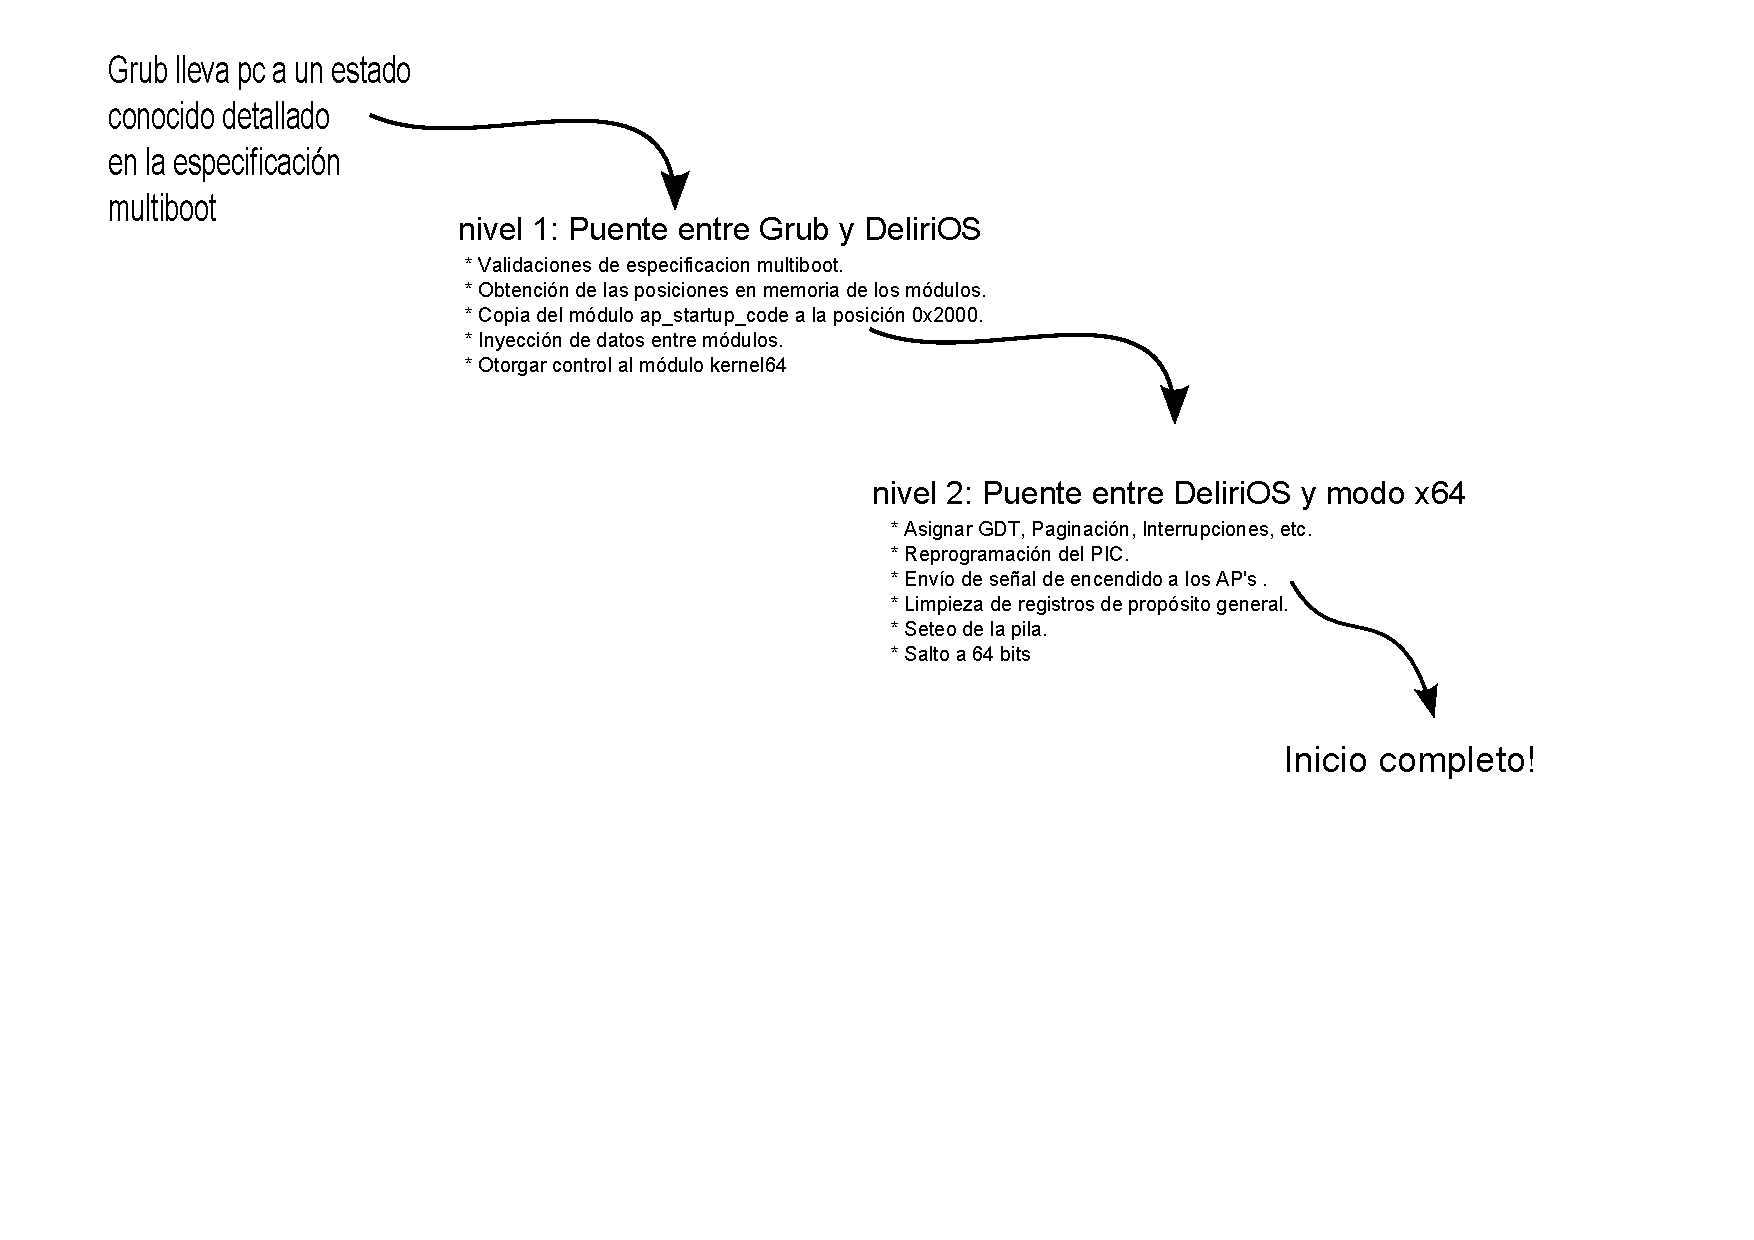
\includegraphics[height=14cm]{images/bsp-stages-diagram.pdf} 
	\end{center}
	
	\subsubsection{Niveles de booteo del AP}

	\begin{center}
		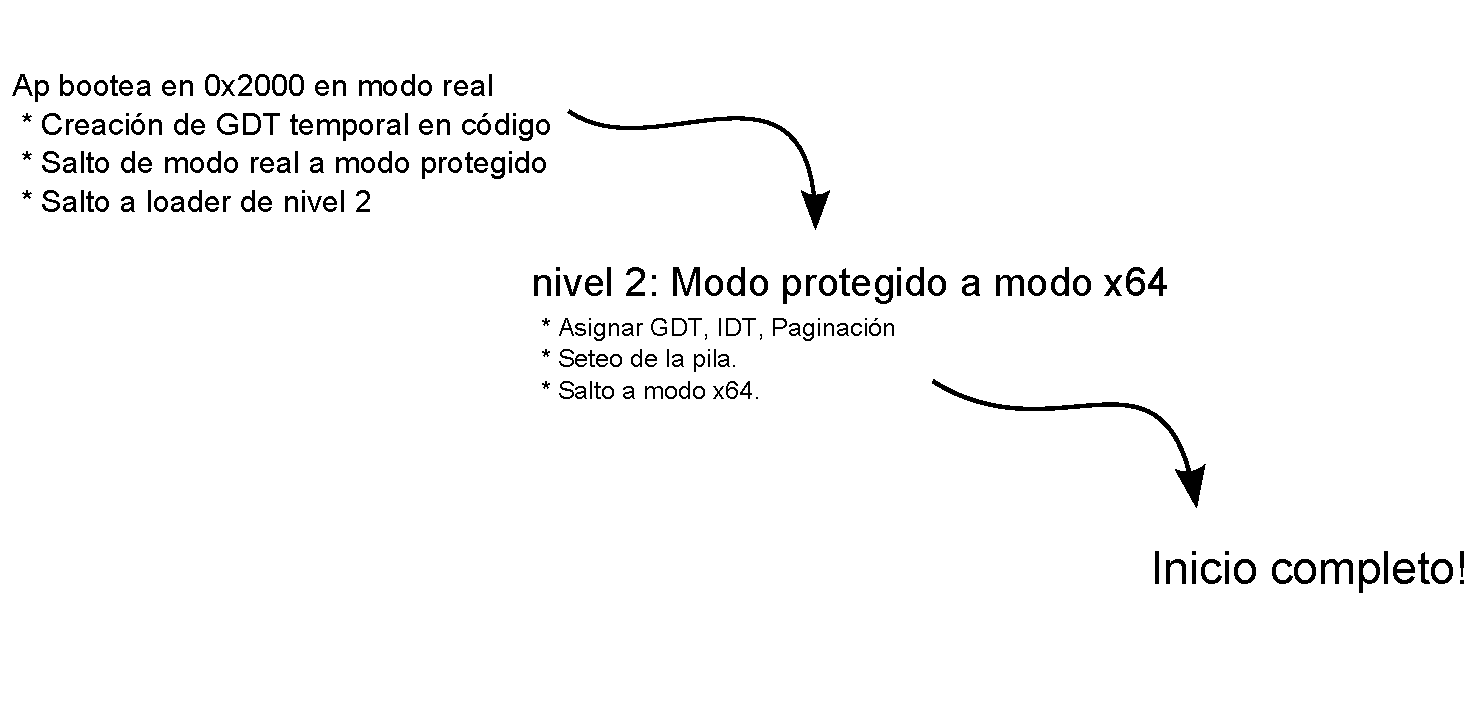
\includegraphics[height=8cm]{images/ap-stages-diagram.pdf} 
	\end{center}

    
        \newpage
        \subsection{Inicialización del Bootstrap processor: Pasaje entre modo protegido a modo legacy x64}
    \subsubsection{Modo Legacy x64: GDT, Paginación de los primeros 4gb}
    La especificación multiboot nos asegura que estamos en modo protegido, pero no tenemos la certeza de tener una GDT válida, es por esto que asignamos una GDT con 
    3 entradas todas de nivel 0, una comun a 32 y 64 bits de datos y 2 de código, esta diferenciación de descriptores de código es necesaria para realizar los jump far para pasar de modo real hacia modo protegido y de modo protegido-compatibilidad x64 hacia modo largo x64.

    TODO: IMAGEN DE LA GDT

    Se utilizó un modelo de paginación en identity mapping donde se cubren los primeros 64 GB de memoria. El modo de paginación elegido fue IA32e en 3 niveles con páginas de 2 megas, es importante remarcar que como para pasar a modo largo de 64 bits es obligatorio tener paginación activa, el mapeo de la memoria virtual fue realizado en 2 etapas, en la primera se mapearon unicamente los primeros 4gb pues desde modo protegido puedo direccionar como máximo hasta 4gb y luego desde modo largo, se completa el esquema de paginacion a 64gb agregando las entradas necesarias a las estructuras.
    \\

    Esquema de paginación IA32-e:

    \begin{itemize}

        \item \textbf{PML4: } 512 entries disponibles de 8 bytes de ancho cada una. Solo fue necesario instanciar la primera entrada de la tabla.

        \item \textbf{PDPT: } 512 entries disponibles de 8 bytes de ancho cada una. 
        Solo fue necesario instanciar las primeras 64 entradas de esta tabla.

        \item \textbf{PDT: } 32768 entries disponibles de 8 bytes de ancho cada una.
        Se instancian en modo protegido 2048 entradas para cubrir los primeros 4gb y luego desde modo largo se completan las 30720 entradas restantes completando 64 gb.
    \end{itemize}

    TODO: IMAGEN DE LOS NIVELES DE PAGINACION CON SUS FLECHITAS MOSTRANDO EN ROJO QUE POR ENCIMA DE 4GB NO SE PUEDE MAPEAR

    TODO: TABLAS CON DIRECCIONES DE LAS ESTRUCTURAS Y CANTIDAD DE ENTRADAS DE CADA UNA.

	Luego de establecer estas estructuras, realizamos una comprobación de disponibilidad de modo x64, y encendemos los bits del procesador para habilitar dicho modo.

    \subsection{Inicialización del Bootstrap processor: Pasaje a modo largo x64 nativo}

    Para pasar de modo compatibilidad a modo nativo de 64 bits, es necesario realizar un salto largo en la ejecucion a un descriptor de la GDT de código de 64 bits.\\
    \\
    Luego de realizar el salto al segmento de código de x64 de la GDT establecemos un contexto seguro con los registros en cero, seteamos los selectores correspondientes de la GDT y establecemos los punteros a una pila asignada al BSP.

    \subsubsection{Modo Largo x64: Extensión de paginación a 64 gb}

    En este punto ya podemos direccionar arriba de los 4gb, entonces completamos las entradas en las estructuras de paginación para completar el mapeo hasta 64gb.

    TODO: IMAGEN DEL MAPEO COMPLETO EN 3 NIVELES

    \subsubsection{Modo Largo x64: Inicialización del PIC - Captura de excepciones e interrupciones}
	
    Enviamos señales al PIC para programarlo de forma que atienda las interrupciones enmascarables y asignamos una IDT que captura todas las excepciones e interrupciones y de ser necesario, realiza las acciones correspondientes con su ISR asociada. Particularmente las excepciones son capturadas y mostradas en pantalla y se utiliza la interrupcion de reloj para sincronizacion y esperas, las demás interrupciones son ignoradas.

    TODO: IMAGEN DE LA IDT Y FLECHITAS A LAS ISR

    \subsubsection{Modo Largo x64: Mapa de memoria del kernel}

    TODO: IMAGEN DEL MAPA DE MEMORIA DEL KERNEL.
    
        \newpage
        \subsection{Multicore: encendido de los AP's}
    \subsubsection{TODO: Ingrese cosas de inicializacion multicore aqui.}    
        \newpage
        \subsection{Multicore: inicialización de modo real a modo nativo x64 de los AP's}
    Como vimos en la sección anterior, los Application Processors comienzan su ejecución en una posición otra por debajo del primer mega en modo real, nosotros necesitamos hacer saltar la ejecución a una posición conocida por encima del mega que no se solape con estructuras del kernel ni otros módulos, la solución que propusimos es un booteo por etapas.
    
    \subsubsection{Booteo por niveles: Modo real a modo protegido y modo protegido en memoria alta}
    En este primer nivel el núcleo se encuentra en modo real, se inicializa una GDT básica en el mismo código y se salta a modo protegido, esto es necesario para poder direccionar posiciones de memoria por encima del primer mega.\\

    Recordando secciones anteriores, cuando el BSP iniciaba el primer nivel de booteo preparaba el contexto de los APS para inicializar en niveles, en este proceso se inyecta en el código del primer nivel de booteo del AP la posicion de memoria donde esta el segundo nivel de booteo por encima del mega.\\

    Luego resta únicamente realizar el salto al segundo bootloader con un jump para continuar el booteo del AP, de manera similar al BSP pasamos luego a modo nativo de 64 bits.\\
    Notemos que por ejemplo la línea A20 ya esta habilitada, y algunas estructuras del kernel que fueron inicializadas por el BSP son comúnes a todos los núcleos, como por ejemplo la GDT y la estructura jerárquica de paginación,
    que son directamente asignadas a los registros del núcleo correspondiente con punteros a ellas.
    \\
    Para el manejo de interrupciones y excepciones, se inicializa una IDT para los Application Processors, además es necesario habilitar los local-apic de cada AP, en caso contrario, no podríamos utilizar interrupciones inter-procesador(IPIS).
    \\

    Como el número de application processors puede ser variable a priori, cuando un núcleo comienza su ejecución, es obtenido su código de identificación dentro del procesador y luego se obtiene una posición de memoria única para cada núcleo con el fin de poder asignar los punteros de la pila $RSP$ y $RBP$, de ser necesaria la reserva de memoria para alguna otra estructura única por núcleo se puede utilizar este recurso.   
        \newpage
    \section{Desarrollo: Algoritmos implementados}
        \subsection{Sorting de arreglos}
    \subsubsection{Conjuntos de numeros pseudoaleatorios utilizados para los experimentos}
    \subsubsection{Implementación con un unico core}
    \subsubsection{Implementación con dos cores: Paralelización del algoritmo}
    \subsubsection{Implementación con dos cores: Sincronización con espera activa}
    \subsubsection{Implementación con dos cores: Sincronización con inter processor interrupts}
    
        \newpage
         \subsection{Modificación de elementos de un arreglo}
    \subsubsection{Saturación del canal de memoria}
        \newpage
            \subsection{Fast Fourier Transform}
        \newpage
        \section{Resultados}
\subsection{Lectura e interpretación de resultados por pantalla}
\subsection{Resultados: Forma de medición}
\subsection{Resultados: Plataformas de testing, incluir fsb, ram,cache, etc }
\subsection{Resultados: Comparación de resultados}

        \newpage
    %%%%%%%%%%%%%%%%%%%%%%%%%%%%%%%%%%%%%%%%%%%%%%%%%%%%%%%%%%%%%%%%%%%%%%%%%%%%%%%
    %% Conclusion                                                                %%
    %%%%%%%%%%%%%%%%%%%%%%%%%%%%%%%%%%%%%%%%%%%%%%%%%%%%%%%%%%%%%%%%%%%%%%%%%%%%%%%
    \section{Conclusión Final}
        Como conclusión de este trabajo, pensamos que la performance obtenida al utilizar dual core a un nivel muy bajo para algoritmos paralelizables no es para nada despreciable, dado que obtuvimos mejoras entre 50\% y 100\% dependiendo de la arquitectura del hardware donde se realizaron los experimentos, esto es una mejor performance que utilizando la infraestructura de threads de lenguajes de alto nivel. Restaría investigar mas aplicaciones en las cuales se pueda aprovechar este modelo ultra eficiente de cómputo y realizar pruebas con sistemas operativos reales que nos permitan verificar que el overhead creado por estos sea suficientemente apreciable como para decidir utilizar nuestra herramienta.

\end{document}